\documentclass{article}
\usepackage[hyphens]{url}
\usepackage{mathtools}
\usepackage{amsmath}
\usepackage{listings}
\usepackage{graphicx}
\usepackage[margin=1in]{geometry}
\usepackage{float}
\floatstyle{boxed}
\restylefloat{figure}
\lstset{breaklines=true}
\begin{document}


\title{CS595 Intro to Web Science, Assignment \#6}
\author{Valentina Neblitt-Jones}
\date{October 31, 2013}
\maketitle



\section*{Question 1}

We know the result of the Karate Club (Zachary, 1977) split. Prove or disprove that the result of split could have been predicted by the weighted graph of social interactions. How well does the mathematical model represent reality? \\

Generously support your answer with all supporting equations, code, graphs, arguments, etc. \\

Useful sources include:  \\

\begin{itemize}
\item Original paper
	\begin{itemize}
	\item \url{http://aris.ss.uci.edu/~lin/76.pdf}
	\end{itemize}
\item Slides 
	\begin{itemize}
	\item \url{http://www-personal.umich.edu/~ladamic/courses/networks/si614w06/ppt/lecture18.ppt}
	\item \url{http://clair.si.umich.edu/si767/papers/Week03/Community/CommunityDetection.pptx}
	\end{itemize}
\item{Code and data}
	\begin{itemize}
	\item \url{http://networkx.github.io/documentation/latest/examples/graph/karate_club.html}
	\item \url{http://nbviewer.ipython.org/url/courses.cit.cornell.edu/info6010/resources/11notes.ipynb}
	\item \url{http://stackoverflow.com/questions/9471906/what-are-the-differences-between-community-detection-algorithms-in-igraph/9478989#9478989}
	\item \url{http://stackoverflow.com/questions/5822265/are-there-implementations-of-algorithms-for-community-detection-in-graphs}
	\item \url{http://konect.uni-koblenz.de/networks/ucidata-zachary}
	\item \url{http://vlado.fmf.uni-lj.si/pub/networks/data/ucinet/ucidata.htm#zachary}
	\end{itemize}
\end{itemize}
\subsection*{Answer to Question 1}


%\begin{figure}[H]
%\centering
%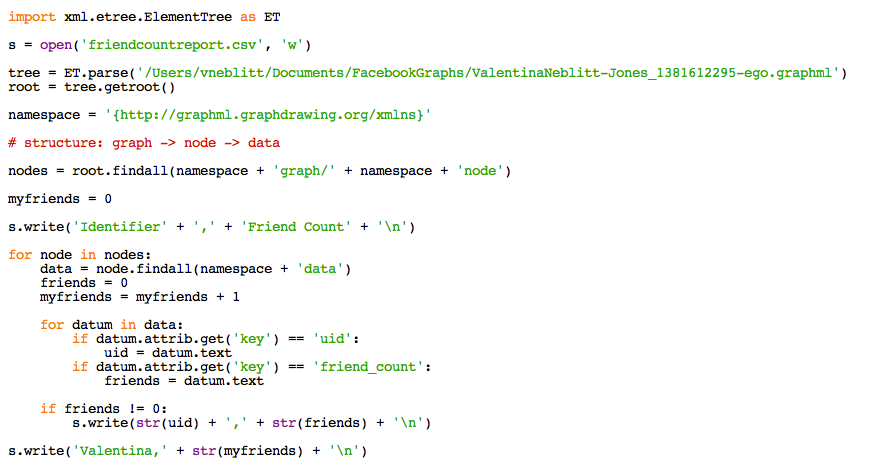
\includegraphics[scale=0.50]{q1/GetFriendCountsCode}
%\caption{Showing Friend Count}
%\label{GetFriendCountsCode}
%\end{figure}

\newpage

\section*{Extra Credit, 3 Points}

We know the group split into two different groups. Suppose the disagreements in the group were more nuanced -- what would the clubs look like if they split into groups of 3, 4, and 5?

%\begin{table}[!h]
%\centering
%\caption{10 Hits for the term ``shadow'', ranked by TFIDF}
%\begin{tabular}{c c c c}
%\hline
%TFIDF & TF & IDF & URI \\
%\hline
%\hline
%0.150 & 0.014 & 10.680 & http://foo.com \\
%0.085 & 0.008 & 10.680 & http://bar.com \\
%\hline
%\end{tabular}
%\end{table}

\subsection*{Answer to Extra Credit}





\newpage

\section*{Resources}

\begin{itemize}
\item Grosfield, Troy. Parsing XML with Python using ElementTree. \url{http://blog.troygrosfield.com/2010/12/18/parsing-xml-with-python-using-elementtree/}
\item McCown, Frank. Producing Simple Graphs with R. \url{http://www.harding.edu/fmccown/r/}
\item Poulson, Barton. R Statistics Essential Training. \url{http://www.lynda.com/course20/R-tutorials/R-Statistics-Essential-Training/142447-2.html}
\item Python.org. The ElementTree XML API. \url{http://docs.python.org/3.3/library/xml.etree.elementtree.html}
\item Seminar for Statistics. R Documentation: Arithmetic Mean. \url{http://stat.ethz.ch/R-manual/R-devel/library/base/html/mean.html}
\item Seminar for Statistics. R Documentation: Concatenate Strings. \url{http://stat.ethz.ch/R-manual/R-devel/library/base/html/paste.html}
\item Seminar for Statistics. R Documentation: Median Value. \url{http://stat.ethz.ch/R-manual/R-patched/library/stats/html/median.html}
\item Seminar for Statistics. R Documentation: Standard Deviation. \url{http://stat.ethz.ch/R-manual/R-patched/library/stats/html/sd.html}
\item Stack Overflow. Change colors or particular bars in a bar chart. \url{http://stackoverflow.com/questions/13112974/change-colours-of-particular-bars-in-a-bar-chart}
\item Stack Overflow. How do you print to stderr in R? \url{http://stackoverflow.com/questions/1109017/how-do-you-print-to-stderr-in-r}
\item Stack Overflow. Understanding the Order() function in R. \url{http://stackoverflow.com/questions/2315601/understanding-the-order-function-in-r}
\item Twitter Developers Documentation. GET followers/list. \url{https://dev.twitter.com/docs/api/1.1/get/followers/list}
\item Twitter Developers Documentation. Using cursors to navigate collections. \url{https://dev.twitter.com/docs/misc/cursoring}
\end{itemize}

\end{document}